\documentclass[dvipdfmx]{jsarticle}
\setcounter{section}{2}
\setcounter{subsection}{1}
\usepackage{xr}
\externaldocument{2.1.2}
\externaldocument{2.1.5}
\externaldocument{2.1.6}
\externaldocument{2.1.11}
\usepackage{amsmath,amsfonts,amssymb,array,comment,mathtools,url,docmute}
\usepackage{longtable,booktabs,dcolumn,tabularx,mathtools,multirow,colortbl,xcolor}
\usepackage[dvipdfmx]{graphics}
\usepackage{bmpsize}
\usepackage{amsthm}
\usepackage{enumitem}
\setlistdepth{20}
\renewlist{itemize}{itemize}{20}
\setlist[itemize]{label=•}
\renewlist{enumerate}{enumerate}{20}
\setlist[enumerate]{label=\arabic*.}
\setcounter{MaxMatrixCols}{20}
\setcounter{tocdepth}{3}
\newcommand{\rotin}{\text{\rotatebox[origin=c]{90}{$\in $}}}
\newcommand{\amap}[6]{\text{\raisebox{-0.7cm}{\begin{tikzpicture} 
  \node (a) at (0, 1) {$\textstyle{#2}$};
  \node (b) at (#6, 1) {$\textstyle{#3}$};
  \node (c) at (0, 0) {$\textstyle{#4}$};
  \node (d) at (#6, 0) {$\textstyle{#5}$};
  \node (x) at (0, 0.5) {$\rotin $};
  \node (x) at (#6, 0.5) {$\rotin $};
  \draw[->] (a) to node[xshift=0pt, yshift=7pt] {$\textstyle{\scriptstyle{#1}}$} (b);
  \draw[|->] (c) to node[xshift=0pt, yshift=7pt] {$\textstyle{\scriptstyle{#1}}$} (d);
\end{tikzpicture}}}}
\newcommand{\twomaps}[9]{\text{\raisebox{-0.7cm}{\begin{tikzpicture} 
  \node (a) at (0, 1) {$\textstyle{#3}$};
  \node (b) at (#9, 1) {$\textstyle{#4}$};
  \node (c) at (#9+#9, 1) {$\textstyle{#5}$};
  \node (d) at (0, 0) {$\textstyle{#6}$};
  \node (e) at (#9, 0) {$\textstyle{#7}$};
  \node (f) at (#9+#9, 0) {$\textstyle{#8}$};
  \node (x) at (0, 0.5) {$\rotin $};
  \node (x) at (#9, 0.5) {$\rotin $};
  \node (x) at (#9+#9, 0.5) {$\rotin $};
  \draw[->] (a) to node[xshift=0pt, yshift=7pt] {$\textstyle{\scriptstyle{#1}}$} (b);
  \draw[|->] (d) to node[xshift=0pt, yshift=7pt] {$\textstyle{\scriptstyle{#2}}$} (e);
  \draw[->] (b) to node[xshift=0pt, yshift=7pt] {$\textstyle{\scriptstyle{#1}}$} (c);
  \draw[|->] (e) to node[xshift=0pt, yshift=7pt] {$\textstyle{\scriptstyle{#2}}$} (f);
\end{tikzpicture}}}}
\renewcommand{\thesection}{第\arabic{section}部}
\renewcommand{\thesubsection}{\arabic{section}.\arabic{subsection}}
\renewcommand{\thesubsubsection}{\arabic{section}.\arabic{subsection}.\arabic{subsubsection}}
\everymath{\displaystyle}
\allowdisplaybreaks[4]
\usepackage{vtable}
\theoremstyle{definition}
\newtheorem{thm}{定理}[subsection]
\newtheorem*{thm*}{定理}
\newtheorem{dfn}{定義}[subsection]
\newtheorem*{dfn*}{定義}
\newtheorem{axs}[dfn]{公理}
\newtheorem*{axs*}{公理}
\renewcommand{\headfont}{\bfseries}
\makeatletter
  \renewcommand{\section}{%
    \@startsection{section}{1}{\z@}%
    {\Cvs}{\Cvs}%
    {\normalfont\huge\headfont\raggedright}}
\makeatother
\makeatletter
  \renewcommand{\subsection}{%
    \@startsection{subsection}{2}{\z@}%
    {0.5\Cvs}{0.5\Cvs}%
    {\normalfont\LARGE\headfont\raggedright}}
\makeatother
\makeatletter
  \renewcommand{\subsubsection}{%
    \@startsection{subsubsection}{3}{\z@}%
    {0.4\Cvs}{0.4\Cvs}%
    {\normalfont\Large\headfont\raggedright}}
\makeatother
\makeatletter
\renewenvironment{proof}[1][\proofname]{\par
  \pushQED{\qed}%
  \normalfont \topsep6\p@\@plus6\p@\relax
  \trivlist
  \item\relax
  {
  #1\@addpunct{.}}\hspace\labelsep\ignorespaces
}{%
  \popQED\endtrivlist\@endpefalse
}
\makeatother
\renewcommand{\proofname}{\textbf{証明}}
\usepackage{tikz,graphics}
\usepackage[dvipdfmx]{hyperref}
\usepackage{pxjahyper}
\hypersetup{
 setpagesize=false,
 bookmarks=true,
 bookmarksdepth=tocdepth,
 bookmarksnumbered=true,
 colorlinks=false,
 pdftitle={},
 pdfsubject={},
 pdfauthor={},
 pdfkeywords={}}
\begin{document}
%\hypertarget{ux56faux6709ux5024}{%
\subsection{固有値}%\label{ux56faux6709ux5024}}
%\hypertarget{ux56faux6709ux5024-1}{%
\subsubsection{固有値}%\label{ux56faux6709ux5024-1}}
\begin{dfn}
以下、体$K$上のvector空間$K^{n}$において、線形写像$f:K^{n} \rightarrow K^{n}$が$f:K^{n} \rightarrow K^{n};\mathbf{v} \mapsto A_{nn}\mathbf{v}$と与えられたとき、その線形写像$f$を$L_{A_{nn}}$とおくことにする。
\end{dfn}
\begin{dfn}
体$K$上のvector空間$V$において、線形写像$f:V \rightarrow V$が与えられたとする。$f\left( \mathbf{v} \right) = \lambda\mathbf{v}$が成り立つような零vectorでないそのvector空間$V$のvector$\mathbf{v}$とその体$K$の元$\lambda$が存在するとき、その元$\lambda$をその線形写像$f$の固有値といい、そのvector$\mathbf{v}$をその線形写像$f$のその固有値$\lambda$に対する固有vectorという。
\end{dfn}
\begin{thm}\label{2.2.2.1}
体$K$上のvector空間$V$において、線形写像$f:V \rightarrow V$の固有値$\alpha$が与えられたとき、vector$\mathbf{v}$がその固有値$\lambda$に対する固有vectorであるなら、$\forall k \in K$に対し、そのvector$k\mathbf{v}$もその固有値$\lambda$に対する固有vectorである。
\end{thm}
\begin{proof}
体$K$上のvector空間$V$において、線形写像$f:V \rightarrow V$の固有値$\lambda$が与えられたとき、vector$\mathbf{v}$がその固有値$\lambda$に対する固有vectorであるなら、$\forall k \in K$に対し、そのvector$k\mathbf{v}$は次のことを満たすので、
\begin{align*}
f\left( k\mathbf{v} \right) = kf\left( \mathbf{v} \right) = k\left( \lambda\mathbf{v} \right) = \lambda\left( k\mathbf{v} \right)
\end{align*}
そのvector$k\mathbf{v}$もその固有値$\lambda$に対する固有vectorである。
\end{proof}
\begin{thm}\label{2.2.2.2}
体$K$上のvector空間$V$において、線形写像$f:V \rightarrow V$が与えられたとき、$\exists\lambda \in K$に対し、その元$\lambda$がその線形写像$f$の固有値であるならそのときに限り、そのvector空間$V$の恒等写像$I_{V}$を用いて線形写像$\lambda I_{V} - f$の核$\ker\left( \lambda I_{V} - f \right)$が零vector以外の元を含む、即ち、$\ker\left( \lambda I_{V} - f \right) \supset \left\{ \mathbf{0} \right\}$が成り立つ。このとき、そのvector空間$V$の元$\mathbf{v}$がその固有値$\lambda$に対する固有vectorであるならそのときに限り、そのvector$\mathbf{v}$はその集合$\ker\left( \lambda I_{V} - f \right) \setminus \left\{ \mathbf{0} \right\}$の元である。
\end{thm}
\begin{proof}
体$K$上のvector空間$V$において、線形写像$f:V \rightarrow V$が与えられたとき、$\exists\lambda \in K$に対し、その元$\lambda$がその線形写像$f$の固有値であるなら、$f\left( \mathbf{v} \right) = \lambda\mathbf{v}$が成り立つような零vectorでないそのvector空間$V$のvector$\mathbf{v}$が存在する。ここで、そのvector空間$V$の恒等写像$I_{V}$を用いて次のようになるので、
\begin{align*}
\mathbf{0} &= f\left( \mathbf{v} \right) - f\left( \mathbf{v} \right)\\
&= \lambda\mathbf{v} - f\left( \mathbf{v} \right)\\
&= \lambda I_{V}\left( \mathbf{v} \right) - f\left( \mathbf{v} \right)\\
&= \left( \lambda I_{V} - f \right)\left( \mathbf{v} \right)
\end{align*}
$\mathbf{v} \in \ker\left( \lambda I_{V} - f \right)$が成り立つ。これにより、線形写像$\lambda I_{V} - f$の核$\ker\left( \lambda I_{V} - f \right)$が零vector以外の元を含む、即ち、$\ker\left( \lambda I_{V} - f \right) \supset \left\{ \mathbf{0} \right\}$が成り立つ。\par
逆に、これが成り立つなら、その核$\ker\left( \lambda I_{V} - f \right)$は空集合でないので、$\mathbf{v} \in \ker\left( \lambda I_{V} - f \right)$なる零vectorでないvector$\mathbf{v}$が存在する。したがって、$\left( \lambda I_{V} - f \right)\left( \mathbf{v} \right) = \mathbf{0}$が成り立つ。これにより、次のようになるので、
\begin{align*}
f\left( \mathbf{v} \right) &= f\left( \mathbf{v} \right) - \lambda I_{V}\left( \mathbf{v} \right) + \lambda I_{V}\left( \mathbf{v} \right)\\
&= - \left( \lambda I_{V}\left( \mathbf{v} \right) - f\left( \mathbf{v} \right) \right) + \lambda I_{V}\left( \mathbf{v} \right)\\
&= - \left( \lambda I_{V} - f \right)\left( \mathbf{v} \right) + \lambda I_{V}\left( \mathbf{v} \right)\\
&= \lambda I_{V}\left( \mathbf{v} \right) = \lambda\mathbf{v}
\end{align*}
そのvector$\mathbf{v}$はまさしくその線形写像$f$のその固有値$\lambda$に対する固有vectorである。\par
このとき、そのvector空間$V$の元$\mathbf{v}$がその固有値$\lambda$に対する固有vectorであるならそのときに限り、そのvector$\mathbf{v}$は零vectorでないかつ、$f\left( \mathbf{v} \right) = \lambda\mathbf{v}$が成り立つ。ここで、次のようになるので、
\begin{align*}
f\left( \mathbf{v} \right) = \lambda\mathbf{v} &\Leftrightarrow \lambda I_{V}\left( \mathbf{v} \right) = f\left( \mathbf{v} \right)\\
&\Leftrightarrow \lambda I_{V}\left( \mathbf{v} \right) - f\left( \mathbf{v} \right) = \mathbf{0}\\
&\Leftrightarrow \left( \lambda I_{V} - f \right)\left( \mathbf{v} \right) = \mathbf{0}\\
&\Leftrightarrow \mathbf{v} \in \ker\left( \lambda I_{V} - f \right)
\end{align*}
これが成り立つならそのときに限り、$\mathbf{v} \in \ker\left( \lambda I_{V} - f \right) \setminus \left\{ \mathbf{0} \right\}$が成り立つ。
\end{proof}
\begin{thm}\label{2.2.2.3}
体$K$上のvector空間$V$において、線形写像$f:V \rightarrow V$が与えられたとき、$\exists\lambda \in K$に対し、その元$\lambda$がその線形写像$f$の固有値であるならそのときに限り、その線形写像$\lambda I_{V} - f$が全単射でない。
\end{thm}\par
なお、線形写像が全単射であるかどうかの判定については次の定理が有用であろう。
\begin{thm*}[定理\ref{2.1.5.16}の再掲]
体$K$上の$n$次元vector空間たち$V$、$W$の基底の1つをそれぞれ$\alpha$、$\beta$とし、それらの基底たち$\alpha 、\beta$に関する線形写像$f:V \rightarrow W$の$[ f]^{\beta}_{\alpha} \in M_{nn}(K)$なる表現行列$[ f]^{\beta}_{\alpha}$を用いて写像$F_{\alpha \rightarrow \beta}$が次式のように定義されれば、
\begin{align*}
F_{\alpha \rightarrow \beta}:L(V,W) \rightarrow M_{nn}(K);f \mapsto [ f]^{\beta}_{\alpha}
\end{align*}
$\forall f \in L(V,W)$に対し、次のことは同値である。
\begin{itemize}
\item
  その写像$f$は線形同型写像である。
\item
  その写像$f$は全射$f:V \twoheadrightarrow W$である。
\item
  その写像$f$は単射$f:V \rightarrowtail W$である。
\item
  $n = {\mathrm{rank} }f = \dim{V(f)}$が成り立つ。
\item
  ${\mathrm{nullity} }f = \dim{\ker f} = 0$が成り立つ。
\item
  それらの基底たち$\alpha$、$\beta$に関する線形写像$f:V \rightarrow W$の表現行列$[ f]^{\beta}_{\alpha}$は正則行列である、即ち、$[ f]^{\beta}_{\alpha} \in {\mathrm{GL} }_{n}(K)$が成り立つ。
\item
  その行列$F_{\alpha \rightarrow \beta}(f)$は正則行列である、即ち、$F_{\alpha \rightarrow \beta}(f) \in {\mathrm{GL} }_{n}(K)$が成り立つ。
\end{itemize}
\end{thm*}
\begin{proof}
体$K$上のvector空間$V$において、線形写像$f:V \rightarrow V$が与えられたとき、$\exists\lambda \in K$に対し、その元$\lambda$がその線形写像$f$の固有値であるならそのときに限り、定理\ref{2.2.2.2}よりそのvector空間$V$の恒等写像$I_{V}$を用いて線形写像$\lambda I_{V} - f$の核$\ker\left( \lambda I_{V} - f \right)$が零vector以外の元を含む、即ち、${\mathrm{nullity} }\left( \lambda I_{V} - f \right) \neq 0$が成り立つ。これが成り立つならそのときに限り、定理\ref{2.1.5.16}よりその線形写像$\lambda I_{V} - f$が線形同型写像でない、即ち、全単射でない。
\end{proof}
%\hypertarget{ux56faux6709ux591aux9805ux5f0f}{%
\subsubsection{固有多項式}%\label{ux56faux6709ux591aux9805ux5f0f}}
\begin{thm}\label{2.2.2.4}
体$K$上の2つの基底たち$\alpha$、$\beta$をもつ$n$次元vector空間$V$において、線形写像$f:V \rightarrow V$が与えられたとき、$\forall a \in K$に対し、そのvector空間$V$の恒等写像$I_{V}$、その基底$\alpha$、$\beta$に関するその線形写像$aI_{V} - f$の表現行列それぞれ$\left[ aI_{V} - f \right]_{\alpha}^{\alpha}$、$\left[ aI_{V} - f \right]_{\beta}^{\beta}$を用いると、次式が成り立つ。
\begin{align*}
\det\left[ aI_{V} - f \right]_{\alpha}^{\alpha} = \det\left[ aI_{V} - f \right]_{\beta}^{\beta}
\end{align*}
\end{thm}
\begin{proof}
体$K$上の2つの基底たち$\alpha$、$\beta$をもつ$n$次元vector空間$V$において、線形写像$f:V \rightarrow V$が与えられたとき、$\forall a \in K$に対し、そのvector空間$V$の恒等写像$I_{V}$、その基底$\alpha$からその基底$\beta$への基底変換行列$\left[ I_{V} \right]^{\beta}_{\alpha}$、その基底$\alpha$に関するその線形写像$f$の表現行列$[ f]_{\alpha}^{\alpha}$、その基底$\beta$に関するその線形写像$f$の表現行列$[ f]_{\beta}^{\beta}$、$n$次単位行列$I_{n}$を用いると、定理\ref{2.1.5.10}より次のようになる。
\begin{align*}
\det\left[ aI_{V} - f \right]_{\alpha}^{\alpha} &= \det\left( a\left[ I_{V} \right]_{\alpha}^{\alpha} - [ f]_{\alpha}^{\alpha} \right)\\
&= \det\left( a\left[ I_{V} \circ I_{V} \circ I_{V} \right]_{\alpha}^{\alpha} - \left[ I_{V} \circ f \circ I_{V} \right]_{\alpha}^{\alpha} \right)\\
&= \det\left( a\left[ I_{V} \right]_{\beta}^{\alpha}\left[ I_{V} \right]_{\beta}^{\beta}\left[ I_{V} \right]_{\alpha}^{\beta} - \left[ I_{V} \right]_{\beta}^{\alpha}[ f]_{\beta}^{\beta}\left[ I_{V} \right]_{\alpha}^{\beta} \right)\\
&= \det\left( a{\left[ I_{V} \right]^{\beta}_{\alpha}}^{- 1}\left[ I_{V} \right]_{\beta}^{\beta}\left[ I_{V} \right]^{\beta}_{\alpha} - {\left[ I_{V} \right]_{\alpha}^{\beta}}^{- 1}[ f]_{\beta}^{\beta}\left[ I_{V} \right]_{\alpha}^{\beta} \right)\\
&= \det\left( {\left[ I_{V} \right]_{\alpha}^{\beta}}^{- 1}a\left[ I_{V} \right]_{\beta}^{\beta}\left[ I_{V} \right]_{\alpha}^{\beta} - {\left[ I_{V} \right]^{\beta}_{\alpha}}^{- 1}[ f]_{\beta}^{\beta}\left[ I_{V} \right]_{\alpha}^{\beta} \right)\\
&= \det\left( {\left[ I_{V} \right]_{\alpha}^{\beta}}^{- 1}\left( a\left[ I_{V} \right]_{\beta}^{\beta} - [ f]_{\beta}^{\beta} \right)\left[ I_{V} \right]_{\alpha}^{\beta} \right)\\
&= \det\left( {\left[ I_{V} \right]_{\alpha}^{\beta}}^{- 1}\left[ aI_{V} - f \right]_{\beta}^{\beta}\left[ I_{V} \right]_{\alpha}^{\beta} \right)\\
&= \det{\left[ I_{V} \right]_{\alpha}^{\beta}}^{- 1}\det\left[ aI_{V} - f \right]_{\beta}^{\beta}\det\left[ I_{V} \right]_{\alpha}^{\beta}\\
&= \frac{1}{\det\left[ I_{V} \right]_{\alpha}^{\beta}}\det\left[ I_{V} \right]_{\alpha}^{\beta}\det\left[ aI_{V} - f \right]_{\beta}^{\beta}\\
&= \det\left[ aI_{V} - f \right]_{\beta}^{\beta}
\end{align*}
\end{proof}
\begin{dfn}
体$K$上の基底$\alpha$をもつ$n$次元vector空間$V$において、線形写像$f:V \rightarrow V$が与えられたとき、そのvector空間$V$の恒等写像$I_{V}$、その基底$\alpha$に関するその線形写像$aI_{V} - f$の表現行列$\left[ aI_{V} - f \right]_{\alpha}^{\alpha}$、$n$次元単位行列$I_{n}$を用いて次式のように写像$\varPhi_{f}$を考える。
\begin{align*}
\varPhi_{f}:K \rightarrow K;a \mapsto \det\left[ aI_{V} - f \right]_{\alpha}^{\alpha}
\end{align*}
この写像$\varPhi_{f}$を固有多項式写像という。
\end{dfn}\par
上記の定理\ref{2.2.2.4}よりその写像$\varPhi_{f}$はそのvector空間$V$の基底に依らないことが分かるであろう。
\begin{thm}\label{2.2.2.5}
体$K$上の基底$\alpha$をもつ$n$次元vector空間$V$において、線形写像$f:V \rightarrow V$の固有多項式写像$\varPhi_{f}$は多項式写像である、即ち、固有多項式$\varPhi_{f}(a)$は$i \in \varLambda_{n} \cup \left\{ 0 \right\}$なるある体の元々$k_{i}$を用いて次式のように表されることができる。
\begin{align*}
\varPhi_{f}(a) = \sum_{i \in \varLambda_{n} \cup \left\{ 0 \right\}} {k_{i}a^{i}}
\end{align*}
これにより、これが定められる多項式環$K[ X]$の多項式$\varPhi_{f}$をその線形写像$f$の固有多項式という。さらに、その固有多項式の$n$次係数$k_{n}$、$n - 1$次係数$k_{n - 1}$、定数項$k_{0}$について、その基底$\alpha$に関するその線形写像$f$の表現行列$[ f]_{\alpha}^{\alpha}$を用いると、次のようになる。
\begin{align*}
k_{n} = 1,\ \ k_{n - 1} = - {\mathrm{tr} }[ f]_{\alpha}^{\alpha},\ \ k_{0} = ( - 1)^{n}\det[ f]_{\alpha}^{\alpha}
\end{align*}
\end{thm}\par
なお、その他の元々$k_{i}$を求めるのは証明の議論についてこれば分かるように困難である。
\begin{proof}
体$K$上の基底$\alpha$をもつ$n$次元vector空間$V$において、線形写像$f:V \rightarrow V$の固有多項式$\varPhi_{f}(a)$は、定義よりそのvector空間$V$の恒等写像$I_{V}$、その基底$\alpha$に関するその線形写像$f$の表現行列$[ f]_{\alpha}^{\alpha}$、$n$次単位行列$I_{n}$を用いると、次式を満たす。
\begin{align*}
\varPhi_{f}(a) = \det\left[ aI_{V} - f \right]_{\alpha}^{\alpha} = \det\left( a\left[ I_{V} \right]_{\alpha}^{\alpha} - [ f]_{\alpha}^{\alpha} \right) = \det\left( aI_{n} - [ f]_{\alpha}^{\alpha} \right)
\end{align*}
ここで、$[ f]_{\alpha}^{\alpha} = \left( a_{ij} \right)_{(i,j) \in \varLambda_{n}^{2}}$と、添数集合$\varLambda_{n}$の置換全体の集合を$\mathfrak{S}_{n}$とおくと、定理\ref{2.1.11.5}より次式が成り立つ。
\begin{align*}
\varPhi_{f}(a) = \det\left( aI_{n} - [ f]_{\alpha}^{\alpha} \right) = \sum_{p \in \mathfrak{S}_{n}} {{\mathrm{sgn} }p\prod_{j \in \varLambda_{n}} \left( a\delta_{p(j)j} - a_{p(j)j} \right)}
\end{align*}
したがって、次のようになる。
\begin{align*}
\varPhi_{f}(a) = \sum_{p \in \mathfrak{S}_{n}} {{\mathrm{sgn} }p\prod_{\scriptsize \begin{matrix} j \in \varLambda_{n} \\ p(j) \neq j \end{matrix}} \left( - a_{p(j)j} \right)\prod_{\scriptsize \begin{matrix} j \in \varLambda_{n} \\ p(j) = j \end{matrix}} \left( a - a_{p(j)j} \right)}
\end{align*}\par
ここで、$j \in \varLambda_{n}$かつ$p(j) = j$が成り立つような添数$j$全体の集合を$\varLambda_{p}'$とおくと、$\# \varLambda_{p}' = L$として、$i \in \varLambda_{L} \cup \left\{ 0 \right\}$なるある体の元々$k_{i}'$を用いて次式を満たすかつ$k_{L}' = 1$かつ$k_{L - 1}' = - \sum_{i \in \varLambda_{p}'} a_{ii}$が成り立つことを示そう。
\begin{align*}
\prod_{\scriptsize \begin{matrix} j \in \varLambda_{n}\\ p(j) = j \\ \end{matrix}} \left( a - a_{p(j)j} \right) = \prod_{j \in \varLambda_{p}'} \left( a - a_{jj} \right) = \sum_{i \in \varLambda_{L} \cup \left\{ 0 \right\}} {k_{i}'a^{i}}
\end{align*}
このとき、$\# \varLambda_{L} \leq \# \varLambda_{n} = n$が成り立つことに注意すれば、$L = 1$のとき、$j' \in \varLambda_{L}$なる添数$j'$を用いれば明らかに$\prod_{j \in \varLambda_{p}'} \left( a - a_{jj} \right) = a - a_{j'j'}$が成り立つ。\par
$1 \leq L = k \leq n - 1$のとき、$\prod_{j \in \varLambda_{p}'} \left( a - a_{jj} \right) = \sum_{i \in \varLambda_{L} \cup \left\{ 0 \right\}} {k_{i}'a^{i}}$が成り立つかつ$k_{k}' = 1$かつ$k_{k - 1}' = - \sum_{i \in \varLambda_{p}'} a_{ii}$が成り立つと仮定しよう。\par
$2 \leq L = k + 1 \leq 1$のとき、あるその集合$\varLambda_{L}$の添数$j'$を用いると、$\# \left( \varLambda_{p}' \setminus \left\{ j' \right\} \right) = k$が成り立つことに注意すれば、仮定より次のようになる。
\begin{align*}
\prod_{j \in \varLambda_{p}'} \left( a - a_{jj} \right) &= \left( a - a_{j'j'} \right)\prod_{j \in \varLambda_{p}' \setminus \left\{ j' \right\}} \left( a - a_{jj} \right)\\
&= \left( a - a_{j'j'} \right)\sum_{i \in \varLambda_{k} \cup \left\{ 0 \right\}} {k_{i}'a^{i}}\\
&= \left( a - a_{j'j'} \right)\left( k_{k}'a^{k} + k_{k - 1}'a^{k - 1} + \sum_{i \in \left( \varLambda_{k} \cup \left\{ 0 \right\} \right) \setminus \left\{ k,k - 1 \right\}} {k_{i}'a^{i}} \right)\\
&= \left( a - a_{j'j'} \right)\left( a^{k} - \sum_{i \in \varLambda_{p}' \setminus \left\{ j' \right\}} a_{ii}a^{k - 1} + \sum_{i \in \left( \varLambda_{k} \cup \left\{ 0 \right\} \right) \setminus \left\{ k,k - 1 \right\}} {k_{i}'a^{i}} \right)\\
&= a^{k + 1} - \sum_{i \in \varLambda_{p}' \setminus \left\{ j' \right\}} a_{ii}a^{k} + \sum_{i \in \left( \varLambda_{k} \cup \left\{ 0 \right\} \right) \setminus \left\{ k,k - 1 \right\}} {k_{i}'a^{i + 1}} - a_{j'j'}a^{k} \\
&\quad + a_{j'j'}\sum_{i \in \varLambda_{p}' \setminus \left\{ j' \right\}} a_{ii}a^{k - 1} - a_{j'j'}\sum_{i \in \left( \varLambda_{k} \cup \left\{ 0 \right\} \right) \setminus \left\{ k,k - 1 \right\}} {k_{i}'a^{i}}\\
&= a^{k + 1} - \sum_{i \in \varLambda_{p}'} a_{ii}a^{k} + \sum_{i \in \left( \varLambda_{k} \cup \left\{ 0 \right\} \right) \setminus \left\{ k,k - 1 \right\}} {k_{i}'a^{i + 1}} \\
&\quad + a_{j'j'}\sum_{i \in \varLambda_{p}' \setminus \left\{ j' \right\}} a_{ii}a^{k - 1} - a_{j'j'}\sum_{i \in \left( \varLambda_{k} \cup \left\{ 0 \right\} \right) \setminus \left\{ k,k - 1 \right\}} {k_{i}'a^{i}}\\
&= a^{k + 1} - \sum_{i \in \varLambda_{p}'} a_{ii}a^{k} + \sum_{i \in \varLambda_{k - 1}} {k_{i - 1}'a^{i}} \\
&\quad + a_{j'j'}\sum_{i \in \varLambda_{p}' \setminus \left\{ j' \right\}} a_{ii}a^{k - 1} - a_{j'j'}\sum_{i \in \varLambda_{k - 1}} {k_{i - 1}'a^{i - 1}}
\end{align*}
以上より、数学的帰納法によって$i \in \varLambda_{L} \cup \left\{ 0 \right\}$なるある体の元々$k_{i}'$を用いて次式を満たすかつ、$k_{\varLambda_{L}}' = 1$かつ$k_{\varLambda_{L} - 1}' = - \sum_{i \in \varLambda_{p}'} a_{ii}$が成り立つことが示された。
\begin{align*}
\prod_{\scriptsize \begin{matrix} j \in \varLambda_{n} \\ p(j) = j \end{matrix}} \left( a - a_{p(j),j} \right) = \prod_{j \in \varLambda_{p}'} \left( a - a_{jj} \right) = \sum_{i \in \varLambda_{L} \cup \left\{ 0 \right\}} {k_{i}'a^{i}}
\end{align*}\par
したがって、次のようになる。
\begin{align*}
\varPhi_{f}(a) &= \sum_{p \in \mathfrak{S}_{n}} {{\mathrm{sgn} }p\prod_{j \in \varLambda_{n} \setminus \varLambda_{p}'} \left( - a_{p(j),j} \right)\sum_{i \in \varLambda_{L} \cup \left\{ 0 \right\}} {k_{i}'a^{i}}}\\
&= \sum_{l \in \varLambda_{n}} {\sum_{\scriptsize \begin{matrix} p \in \mathfrak{S}_{n} \\ L = l \\\end{matrix}} {{\mathrm{sgn} }p\prod_{j \in \varLambda_{n} \setminus \varLambda_{p}' ,\ } \left( - a_{p(j),j} \right)\sum_{i \in \varLambda_{L} \cup \left\{ 0 \right\}} {k_{i}'a^{i}}}}\\
&= \sum_{\scriptsize \begin{matrix} p \in \mathfrak{S}_{n} \\ L = n\\\end{matrix}} {{\mathrm{sgn} }p\prod_{j \in \varLambda_{n} \setminus \varLambda_{p}' ,\ } \left( - a_{p(j),j} \right)\sum_{i \in \varLambda_{L} \cup \left\{ 0 \right\}} {k_{i}'a^{i}}} \\
&\quad + \sum_{l \in \varLambda_{n - 1}} {\sum_{\scriptsize \begin{matrix} p \in \mathfrak{S}_{n} \\ L = l \\\end{matrix}} {{\mathrm{sgn} }p\prod_{j \in \varLambda_{n} \setminus \varLambda_{p}' } \left( - a_{p(j),j} \right)\sum_{i \in \varLambda_{l} \cup \left\{ 0 \right\}} {k_{i}'a^{i}}}}
\end{align*}
ここで、次のようになるので、
\begin{align*}
\sum_{\scriptsize \begin{matrix} p \in \mathfrak{S}_{n} \\ L = n\\\end{matrix}} {{\mathrm{sgn} }p\prod_{j \in \varLambda_{n} \setminus \varLambda_{p}' } \left( - a_{p(j),j} \right)\sum_{i \in \varLambda_{L} \cup \left\{ 0 \right\}} {k_{i}'a^{i}}} &= \sum_{p = I_{\varLambda_{n}}} {{\mathrm{sgn} }p\prod_{j \in \varLambda_{n} \setminus \varLambda_{p}' } \left( - a_{p(j),j} \right)\sum_{i \in \varLambda_{L} \cup \left\{ 0 \right\}} {k_{i}'a^{i}}}\\
&= \sum_{p = I_{\varLambda_{n}}} {{\mathrm{sgn} }I_{\varLambda_{n}}\prod_{j \in \varLambda_{n} \setminus \varLambda_{I_{\varLambda_{n}}}' } \left( - a_{p(j),j} \right)\sum_{i \in \varLambda_{n} \cup \left\{ 0 \right\}} {k_{i}'a^{i}}}\\
&= \prod_{j \in \emptyset } \left( - a_{p(j),j} \right)\sum_{i \in \varLambda_{n} \cup \left\{ 0 \right\}} {k_{i}'a^{i}} = \sum_{i \in \varLambda_{n} \cup \left\{ 0 \right\}} {k_{i}'a^{i}}
\end{align*}
したがって、次のようになる。
\begin{align*}
\varPhi_{f}(a) = \sum_{i \in \varLambda_{n} \cup \left\{ 0 \right\}} {k_{i}'a^{i}} + \sum_{l \in \varLambda_{n - 1}} {\sum_{\scriptsize \begin{matrix} p \in \mathfrak{S}_{n} \\ L = l \\\end{matrix}} {{\mathrm{sgn} }p\prod_{j \in \varLambda_{n} \setminus \varLambda_{p}' } \left( - a_{p(j),j} \right)\sum_{i \in \varLambda_{l} \cup \left\{ 0 \right\}} {k_{i}'a^{i}}}}
\end{align*}\par
ここで、$L = n - 1$なる置換$p$が存在すると仮定すると、ある1つの添数$j'$に対してのみ$p\left( j' \right) \neq j'$が成り立ちその添数$j'$以外の添数$j$では$p(j) = j$が成り立つことになる。このとき、その置換は全単射なので、逆写像$p^{- 1}$が存在して$p^{- 1}\left( p\left( j' \right) \right) = j'$が成り立つかつ、$p\left( j'' \right) = p\left( j' \right)$なるその添数$j'$とは異なる添数$j''$が存在して$p\left( j' \right) = j''$が成り立つことになる。したがって、次のようになる。
\begin{align*}
j' = p^{- 1}\left( p\left( j' \right) \right) = p^{- 1}\left( j'' \right) = j''
\end{align*}
しかしながら、これは仮定に矛盾する。\par
したがって、$L = n - 1$なる置換$p$が存在しないことになるので、次のようになる。
\begin{align*}
\varPhi_{f}(a) &= \sum_{i \in \varLambda_{n} \cup \left\{ 0 \right\}} {k_{i}'a^{i}} + \sum_{l \in \varLambda_{n - 2}} {\sum_{\scriptsize \begin{matrix} p \in \mathfrak{S}_{n} \\ L = l \\\end{matrix}} {{\mathrm{sgn} }p\prod_{j \in \varLambda_{n} \setminus \varLambda_{p}' } \left( - a_{p(j),j} \right)\sum_{i \in \varLambda_{l} \cup \left\{ 0 \right\}} {k_{i}'a^{i}}}}\\
&= k_{n}'a^{n} + k_{n - 1}'a^{n - 1} + \sum_{i \in \left( \varLambda_{n} \cup \left\{ 0 \right\} \right) \setminus \left\{ n,n - 1 \right\}} {k_{i}'a^{i}} \\
&\quad + \sum_{l \in \varLambda_{n - 2}} {\sum_{\scriptsize \begin{matrix} p \in \mathfrak{S}_{n} \\ L = l \\\end{matrix}} {{\mathrm{sgn} }p\prod_{j \in \varLambda_{n} \setminus \varLambda_{p}' } \left( - a_{p(j),j} \right)\sum_{i \in \varLambda_{l} \cup \left\{ 0 \right\}} {k_{i}'a^{i}}}}\\
&= k_{n}'a^{n} + k_{n - 1}'a^{n - 1} + \sum_{i \in \varLambda_{n - 2} \cup \left\{ 0 \right\}} {k_{i}'a^{i}} \\
&\quad + \sum_{l \in \varLambda_{n - 2}} {\sum_{\scriptsize \begin{matrix} p \in \mathfrak{S}_{n}\\ L = l \end{matrix}} {{\mathrm{sgn} }p\prod_{j \in \varLambda_{n} \setminus \varLambda_{p}' } \left( - a_{p(j),j} \right)\sum_{i \in \varLambda_{l} \cup \left\{ 0 \right\}} {k_{i}'a^{i}}}}
\end{align*}
ここで、$i \in \varLambda_{n} \cup \left\{ 0 \right\}$なるある体の元々$k_{i}$を用いれば、$k_{n} = k_{n}' = 1$かつ$k_{n - 1} = k_{n - 1}' = - \sum_{i \in \varLambda_{n}} a_{ii}$かつ次式を満たすので、
\begin{align*}
\sum_{i \in \varLambda_{n - 2} \cup \left\{ 0 \right\}} {k_{i}'a^{i}} + \sum_{l \in \varLambda_{n - 2}} {\sum_{\scriptsize \begin{matrix} p \in \mathfrak{S}_{n}\\ L = l \\\end{matrix}} {{\mathrm{sgn} }p\prod_{j \in \varLambda_{n} \setminus \varLambda_{p}' } \left( - a_{p(j),j} \right)\sum_{i \in \varLambda_{l} \cup \left\{ 0 \right\}} {k_{i}'a^{i}}}} = \sum_{i \in \varLambda_{n - 2} \cup \left\{ 0 \right\}} {k_{i}a^{i}}
\end{align*}
次式が得られる。
\begin{align*}
\varPhi_{f}(a) = \sum_{i \in \varLambda_{n} \cup \left\{ 0 \right\}} {k_{i}a^{i}}
\end{align*}
さらに、それらの元々$k_{n}$、$k_{n - 1}$は次式を満たす。
\begin{align*}
k_{n} = 1,\ \ k_{n - 1} = - \sum_{i \in \varLambda_{n}} a_{ii} = - {\mathrm{tr} }[ f]_{\alpha}^{\alpha}
\end{align*}\par
また、その線形写像$f$の固有多項式写像$\varPhi_{f}$の0による像について考えよう。このとき、その基底$\alpha$に関するその線形写像$f$の表現行列$[ f]_{\alpha}^{\alpha}$を用いて次のようになるかつ、
\begin{align*}
\varPhi_{f}(0) = \det\left[ 0I_{V} - f \right]_{\alpha}^{\alpha} = \det\left( - [ f]_{\alpha}^{\alpha} \right) = ( - 1)^{n}\det[ f]_{\alpha}^{\alpha}
\end{align*}
上記の議論により$i \in \varLambda_{n} \cup \left\{ 0 \right\}$なるある体の元々$k_{i}$を用いて次式を満たすので、
\begin{align*}
\varPhi_{f}(a) = \sum_{i \in \varLambda_{n} \cup \left\{ 0 \right\}} {k_{i}a^{i}} = \sum_{i \in \varLambda_{n}} {k_{i}a^{i}} + k_{0}
\end{align*}
次のようになる。
\begin{align*}
\varPhi_{f}(0) = \sum_{i \in \varLambda_{n}} {k_{i}0^{i}} + k_{0} = k_{0}
\end{align*}
以上より、$k_{0} = ( - 1)^{n}\det[ f]_{\alpha}^{\alpha}$が得られる。
\end{proof}
\begin{thm}\label{2.2.2.6}
体$K$上の$n$次元vector空間$V$において、線形写像$f:V \rightarrow V$が与えられたとき、$\exists\lambda \in K$に対し、その元$\lambda$がその線形写像$f$の固有値であるならそのときに限り、その元$\lambda$がその線形写像$f$の固有多項式の根である。
\end{thm}\par
ここで、例えば、$K = \mathbb{R}$が成り立つとき、$\varPhi_{f}(\lambda) = 0$が成り立つようなその元$\lambda$は実数でなければならないことになることに注意されたい。
\begin{proof}
体$K$上の$n$次元vector空間$V$において、線形写像$f:V \rightarrow V$が与えられたとき、$\exists\lambda \in K$に対し、その元$\lambda$がその線形写像$f$の固有値であるならそのときに限り、定理\ref{2.1.11.15}、定理\ref{2.1.5.16}、定理\ref{2.2.2.3}よりその線形写像$\lambda I_{V} - f$の表現行列$\left[ \lambda I_{V} - f \right]_{\alpha}^{\alpha}$について、$\det\left[ \lambda I_{V} - f \right]_{\alpha}^{\alpha} = 0$が成り立つ。これは定義よりその線形写像$f$の固有多項式写像$\varPhi_{f}$のその元$\lambda$による像が0に等しい、即ち、その元$\lambda$がその線形写像$f$の固有多項式の根であることと同値である。
\end{proof}
\begin{thm}\label{2.2.2.7}
$A_{nn} \in M_{nn}(K)$なる体$K$上の行列$A_{nn}$が次式を満たすなら、
\begin{align*}
A_{nn} = \begin{pmatrix}
a_{11} & a_{12} & \cdots & a_{1n} \\
\  & a_{22} & \cdots & a_{2n} \\
\  & \  & \ddots & \vdots \\
O & \  & \  & a_{nn} \\
\end{pmatrix}
\end{align*}
体$K$上の$n$次元vector空間$V$において、そのvector空間$V$の基底$\alpha$に関する線形写像$f:V \rightarrow V$の表現行列が$A_{nn}$であるようなその線形写像$f$の固有多項式$\varPhi_{f}$について、次式が成り立つ。
\begin{align*}
\varPhi_{f} = \prod_{i \in \varLambda_{n}} \left( X - a_{ii} \right)
\end{align*}
\end{thm}
\begin{proof}
$A_{nn} \in M_{nn}(K)$なる体$K$上の行列$A_{nn}$が次式を満たすなら、
\begin{align*}
A_{nn} = \begin{pmatrix}
a_{11} & a_{12} & \cdots & a_{1n} \\
\  & a_{22} & \cdots & a_{2n} \\
\  & \  & \ddots & \vdots \\
O & \  & \  & a_{nn} \\
\end{pmatrix}
\end{align*}
体$K$上の$n$次元vector空間$V$において、そのvector空間$V$の基底$\alpha$に関する線形写像$f:V \rightarrow V$の表現行列が$A_{nn}$であるようなその線形写像$f$の固有多項式写像$\varPhi_{f}$について、$\forall a \in K$に対し、定義よりそのvector空間$V$の恒等写像$I_{V}$、$n$次単位行列$I_{n}$を用いて次のようになる。
\begin{align*}
\varPhi_{f}(a) &= \det\left[ aI_{V} - f \right]_{\alpha}^{\alpha}\\
&= \det\left( a\left[ I_{V} \right]_{\alpha}^{\alpha} - [ f]_{\alpha}^{\alpha} \right)\\
&= \det\left( aI_{n} - A_{nn} \right)\\
&= \left| \begin{matrix}
a - a_{11} & a_{12} & \cdots & a_{1n} \\
\  & a - a_{22} & \cdots & a_{2n} \\
\  & \  & \ddots & \vdots \\
O & \  & \  & a - a_{nn} \\
\end{matrix} \right|
\end{align*}
ここで、定理\ref{2.1.11.9}と定理\ref{2.1.11.10}より次式が得られる。
\begin{align*}
\varPhi_{f} = \prod_{i \in \varLambda_{n}} \left( X - a_{ii} \right)
\end{align*}
\end{proof}
\begin{thm}\label{2.2.2.8}
$A_{nn} \in M_{nn}(K)$なる体$K$上の行列$A_{nn}$が$A' \in M_{rr}(K)$、$A'' \in M_{n - r,n - r}(K)$なる行列たち$A_{rr}$、$A_{n - r,n - r}$を用いて次式のうちいづれかを満たすなら、
\begin{align*}
A_{nn} = \begin{pmatrix}
A' & * \\
O & A'' \\
\end{pmatrix},\ \ A_{nn} = \begin{pmatrix}
A' & O \\
* & A'' \\
\end{pmatrix}
\end{align*}
その体$K$上の$n$次元vector空間$V$において、そのvector空間$V$の基底$\alpha$に関する線形写像$f:V \rightarrow V$の表現行列が$A_{nn}$であるようなその線形写像$f$の固有多項式$\varPhi_{f}$について、$\varPhi_{f} = \varPhi_{L_{A'}}\varPhi_{L_{A''}}$が成り立つ。
\end{thm}
\begin{proof}
$A_{nn} \in M_{nn}(K)$なる体$K$上の行列$A_{nn}$が$A' \in M_{rr}(K)$、$A'' \in M_{n - r,n - r}(K)$なる行列たち$A'$、$A''$を用いて次式を満たすなら、
\begin{align*}
A_{nn} = \begin{pmatrix}
A' & * \\
O & A'' \\
\end{pmatrix}
\end{align*}
その体$K$上の$n$次元vector空間$V$において、そのvector空間$V$の基底$\alpha$に関する線形写像$f:V \rightarrow V$の表現行列が$A_{nn}$であるようなその線形写像$f$の固有多項式写像$\varPhi_{f}$について、$\forall a \in K$に対し、定義より$n$次単位行列$I_{n}$、$r$次単位行列$I_{r}$、$n - r$次単位行列$I_{n - r}$を用いて定理\ref{2.1.11.9}と定理\ref{2.1.11.10}より次式が成り立つ。
\begin{align*}
\varPhi_{f}(a) &= \det\left[ aI_{V} - f \right]_{\alpha}^{\alpha}\\
&= \det\left( a\left[ I_{V} \right]_{\alpha}^{\alpha} - [ f]_{\alpha}^{\alpha} \right)\\
&= \det\left( aI_{n} - A_{nn} \right)\\
&= \det\left( a\begin{pmatrix}
I_{r} & O \\
O & I_{n - r} \\
\end{pmatrix} - \begin{pmatrix}
A' & * \\
O & A'' \\
\end{pmatrix} \right)\\
&= \det\begin{pmatrix}
aI_{r} - A' & * \\
O & aI_{n - r} - A'' \\
\end{pmatrix}\\
&= \det\left( aI_{r} - A' \right)\det\left( aI_{n - r} - A'' \right)
\end{align*}
ここで、標準直交基底$\varepsilon$、線形写像たち$L_{A'}$、$L_{A''}$を用いれば、次のようになる。
\begin{align*}
\varPhi_{f}(a) &= \det\left( aI_{r} - A' \right)\det\left( aI_{n - r} - A'' \right)\\
&= \det\left( a\left[ I_{K^{r}} \right]_{\varepsilon}^{\varepsilon} - \left[ L_{A'} \right]_{\varepsilon}^{\varepsilon} \right)\det\left( a\left[ I_{K^{n - r}} \right]_{\varepsilon}^{\varepsilon} - \left[ L_{A''} \right]_{\varepsilon}^{\varepsilon} \right)\\
&= \det\left[ aI_{K^{r}} - L_{A'} \right]_{\varepsilon}^{\varepsilon}\det\left[ aI_{K^{r}} - L_{A''} \right]_{\varepsilon}^{\varepsilon}\\
&= \varPhi_{L_{A'}}(a)\varPhi_{L_{A''}}(a)
\end{align*}\par
$A_{nn} \in M_{nn}(K)$なる体$K$上の行列$A_{nn}$が$A' \in M_{rr}(K)$、$A'' \in M_{n - r,n - r}(K)$なる行列たち$A'$、$A''$を用いて次式を満たすときも同様にして示される。
\begin{align*}
A_{nn} = \begin{pmatrix}
A' & O \\
* & A'' \\
\end{pmatrix}
\end{align*}\par
よって、$\varPhi_{f} = \varPhi_{L_{A'}}\varPhi_{L_{A''}}$が成り立つ。
\end{proof}
\begin{thm}\label{2.2.2.9}
体$K$上の$n$次元vector空間たち$V$、$W$において、線形写像たち$f:V \rightarrow V$、$g:W \rightarrow V$が与えられたとする。その線形写像$g$が線形同型写像であるとき、$\varPhi_{g^{- 1} \circ f \circ g} = \varPhi_{f}$が成り立つ。
\end{thm}
\begin{proof}
体$K$上の$n$次元vector空間たち$V$、$W$において、そのvector空間$V$の基底$\alpha$に関する線形写像たち$f:V \rightarrow V$、$g:W \rightarrow V$が与えられたとする。その線形写像$g$が線形同型写像であるとき、$\forall a \in K$に対し、そのvector空間たち$V$、$W$の恒等写像たち$I_{V}$、$I_{W}$、そのvector空間$V$の基底$\alpha$、そのvector空間の基底$\beta$が与えられたとき、次のようになる。
\begin{align*}
\varPhi_{g^{- 1} \circ f \circ g}(a) &= \det\left[ aI_{W} - g^{- 1} \circ f \circ g \right]_{\beta}^{\beta}\\
&= \det\left[ ag^{- 1} \circ I_{V} \circ g - g^{- 1} \circ f \circ g \right]_{\beta}^{\beta}\\
&= \det\left( a\left[ g^{- 1} \circ I_{V} \circ g \right]_{\beta}^{\beta} - \left[ g^{- 1} \circ f \circ g \right]_{\beta}^{\beta} \right)\\
&= \det\left( a\left[ g^{- 1} \right]^{\beta}_{\alpha}\left[ I_{V} \right]_{\alpha}^{\alpha}[ g]^{\alpha}_{\beta} - \left[ g^{- 1} \right]^{\beta}_{\alpha}[ f]_{\alpha}^{\alpha}[ g]^{\alpha}_{\beta} \right)\\
&= \det{\left[ g^{- 1} \right]^{\beta}_{\alpha}\left( a\left[ I_{V} \right]_{\alpha}^{\alpha} - [ f]_{\alpha}^{\alpha} \right)[ g]^{\alpha}_{\beta}}\\
&= \det\left[ g^{- 1} \right]^{\beta}_{\alpha}\det\left( a\left[ I_{V} \right]_{\alpha}^{\alpha} - [ f]_{\alpha}^{\alpha} \right)\det[ g]^{\alpha}_{\beta}\\
&= \det{[ g]^{\alpha}_{\beta}}^{- 1}\det\left[ aI_{V} - f \right]_{\alpha}^{\alpha}\det[ g]^{\alpha}_{\beta}\\
&= \frac{1}{\det[ g]^{\alpha}_{\beta}}\det[ g]^{\alpha}_{\beta}\det\left[ aI_{V} - f \right]_{\alpha}^{\alpha}\\
&= \det\left[ aI_{V} - f \right]_{\alpha}^{\alpha} = \varPhi_{f}(a)
\end{align*}
よって、$\varPhi_{g^{- 1} \circ f \circ g} = \varPhi_{f}$が成り立つ。
\end{proof}
\begin{thm}\label{2.2.2.10}
体$K$上の$n$次元vector空間$V$において、そのvector空間$V$の線形写像たち$f:V \rightarrow V$、$g:V \rightarrow V$の合成写像たち$g \circ f$、$f \circ g$の固有多項式たちそれぞれ$\varPhi_{g \circ f}$、$\varPhi_{f \circ g}$について、$\varPhi_{g \circ f} = \varPhi_{f \circ g}$が成り立つ。
\end{thm}
\begin{proof}
体$K$上の$n$次元vector空間$V$において、そのvector空間$V$の基底$\alpha$に関する線形写像たち$f:V \rightarrow V$、$g:V \rightarrow V$の合成写像たち$g \circ f$、$f \circ g$の固有多項式写像たちそれぞれ$\varPhi_{g \circ f}$、$\varPhi_{f \circ g}$について、そのvector空間$V$の基底$\alpha$に関するそれらの線形写像たち$f$、$g$の表現行列たちそれぞれ$[ f]_{\alpha}^{\alpha}$、$[ g]_{\alpha}^{\alpha}$とおく。定理\ref{2.1.6.6}より$\exists P,Q \in {\mathrm{GL} }_{n}(K)$に対し、${\mathrm{rank} }[ g]_{\alpha}^{\alpha} = r$とおくと、$r$次単位行列$I_{r}$を用いて次式が成り立つ。
\begin{align*}
P[ g]_{\alpha}^{\alpha}Q^{- 1} = \begin{pmatrix}
I_{r} & O \\
O & O \\
\end{pmatrix}
\end{align*}
このとき、その行列$P[ g]_{\alpha}^{\alpha}Q^{- 1}$、行列$Q[ f]_{\alpha}^{\alpha}P^{- 1}$をそれぞれ$A$、$B$とおくと、定理\ref{2.1.5.1}よりその基底$\alpha$に関する基底変換における線形同型写像$\varphi_{\alpha}:K^{n} \rightarrow V$は全単射で次式のようになる。
\begin{center}
  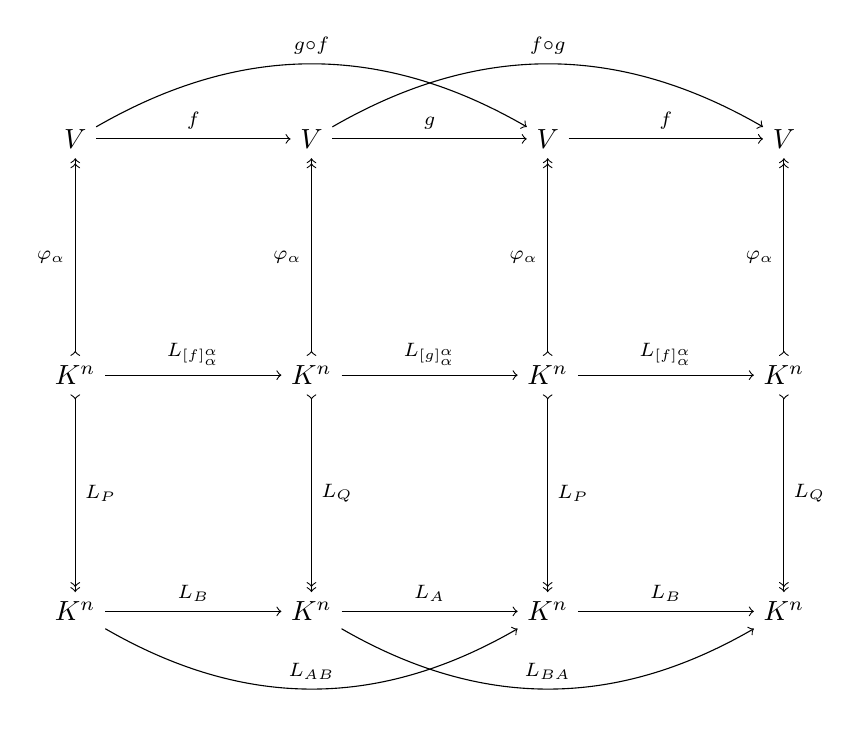
\begin{tikzpicture}[auto]

    \node (a) at (0, 0) {$K^n $};
    \node (b) at (3, 0) {$K^n $};
    \node (c) at (6, 0) {$K^n $};
    \node (d) at (9, 0) {$K^n $};
    \node (e) at (0, 3) {$K^n $};
    \node (f) at (3, 3) {$K^n $};
    \node (g) at (6, 3) {$K^n $};
    \node (h) at (9, 3) {$K^n $};
    \node (i) at (0, 6) {$V$};
    \node (j) at (3, 6) {$V$};
    \node (k) at (6, 6) {$V$};
    \node (l) at (9, 6) {$V$};
    
    \draw [->] (a) to node {$\scriptstyle L_B $} (b);
    \draw [->] (b) to node {$\scriptstyle L_A $} (c);
    \draw [->] (c) to node {$\scriptstyle L_B $} (d);
    \draw [>->>] (e) to node {$\scriptstyle L_P $} (a);
    \draw [>->>] (f) to node {$\scriptstyle L_Q $} (b);
    \draw [>->>] (g) to node {$\scriptstyle L_P $} (c);
    \draw [>->>] (h) to node {$\scriptstyle L_Q $} (d);
    \draw [->] (e) to node {$\scriptstyle L_{\left[ f\right]_{\alpha }^{\alpha }} $} (f);
    \draw [->] (f) to node {$\scriptstyle L_{\left[ g\right]_{\alpha }^{\alpha }} $} (g);
    \draw [->] (g) to node {$\scriptstyle L_{\left[ f\right]_{\alpha }^{\alpha }} $} (h);
    \draw [>->>] (e) to node {$\scriptstyle \varphi_{\alpha } $} (i);
    \draw [>->>] (f) to node {$\scriptstyle \varphi_{\alpha } $} (j);
    \draw [>->>] (g) to node {$\scriptstyle \varphi_{\alpha } $} (k);
    \draw [>->>] (h) to node {$\scriptstyle \varphi_{\alpha } $} (l);
    \draw [->] (i) to node {$\scriptstyle f$} (j);
    \draw [->] (j) to node {$\scriptstyle g$} (k);
    \draw [->] (k) to node {$\scriptstyle f$} (l);
    \draw [->] (a) to [bend right=30] node {$\scriptstyle L_{AB} $} (c);
    \draw [->] (b) to [bend right=30] node {$\scriptstyle L_{BA} $} (d);
    \draw [->] (i) to [bend left=30] node {$\scriptstyle g\circ f$} (k);
    \draw [->] (j) to [bend left=30] node {$\scriptstyle f\circ g$} (l);
  
  \end{tikzpicture}
\end{center}
したがって、次のようになるので、
\begin{align*}
L_{AB} &= L_{P[ g]_{\alpha}^{\alpha}Q^{- 1}Q[ f]_{\alpha}^{\alpha}P^{- 1}}\\
&= L_{P[ g]_{\alpha}^{\alpha}[ f]_{\alpha}^{\alpha}P^{- 1}}\\
&= L_{P[ g \circ f]_{\alpha}^{\alpha}P^{- 1}}\\
&= L_{P} \circ L_{[ g \circ f]_{\alpha}^{\alpha}} \circ L_{P^{- 1}}\\
&= L_{P} \circ L_{[ g \circ f]_{\alpha}^{\alpha}} \circ L_{P}^{- 1}\\
&= L_{P} \circ \varphi_{\alpha}^{- 1} \circ g \circ f \circ \varphi_{\alpha} \circ L_{P}^{- 1}\\
&= \left( L_{P} \circ \varphi_{\alpha}^{- 1} \right) \circ (g \circ f) \circ \left( L_{P} \circ \varphi_{\alpha}^{- 1} \right)^{- 1}, \\
L_{BA} &= L_{Q[ f]_{\alpha}^{\alpha}P^{- 1}P[ g]_{\alpha}^{\alpha}Q^{- 1}}\\
&= L_{Q[ f]_{\alpha}^{\alpha}[ g]_{\alpha}^{\alpha}Q^{- 1}}\\
&= L_{Q[ f \circ g]_{\alpha}^{\alpha}Q^{- 1}}\\
&= L_{Q} \circ L_{[ f \circ g]_{\alpha}^{\alpha}} \circ L_{Q^{- 1}}\\
&= L_{Q} \circ L_{[ f \circ g]_{\alpha}^{\alpha}} \circ L_{Q}^{- 1}\\
&= L_{Q} \circ \varphi_{\alpha}^{- 1} \circ f \circ g \circ \varphi_{\alpha} \circ L_{Q}^{- 1}\\
&= \left( L_{Q} \circ \varphi_{\alpha}^{- 1} \right) \circ (f \circ g) \circ \left( L_{Q} \circ \varphi_{\alpha}^{- 1} \right)^{- 1}
\end{align*}
次式が成り立つ。
\begin{align*}
\varPhi_{L_{AB}} = \varPhi_{\left( L_{P} \circ \varphi_{\alpha}^{- 1} \right) \circ (g \circ f) \circ \left( L_{P} \circ \varphi_{\alpha}^{- 1} \right)^{- 1}},\ \ \varPhi_{L_{BA}} = \varPhi_{\left( L_{Q} \circ \varphi_{\alpha}^{- 1} \right) \circ (f \circ g) \circ \left( L_{Q} \circ \varphi_{\alpha}^{- 1} \right)^{- 1}}
\end{align*}
これは多項式とみても成り立つ。ここで、定理\ref{2.2.2.9}より次のようになる。
\begin{align*}
\varPhi_{L_{AB}} = \varPhi_{g \circ f},\ \ \varPhi_{L_{BA}} = \varPhi_{f \circ g}
\end{align*}\par
また、$B' \in M_{rr}(K)$として行列$B$を次式のようにおくと、
\begin{align*}
B = \begin{pmatrix}
B' & * \\
* & * \\
\end{pmatrix}
\end{align*}
したがって、次のようになる。
\begin{align*}
AB &= \begin{pmatrix}
I_{r} & O \\
O & O \\
\end{pmatrix}\begin{pmatrix}
B' & * \\
* & * \\
\end{pmatrix} = \begin{pmatrix}
B' & * \\
O & O \\
\end{pmatrix}, \\
BA &= \begin{pmatrix}
B' & * \\
* & * \\
\end{pmatrix}\begin{pmatrix}
I_{r} & O \\
O & O \\
\end{pmatrix} = \begin{pmatrix}
B' & O \\
* & O \\
\end{pmatrix}
\end{align*}
ここで、定理\ref{2.2.2.8}より次のようになる。
\begin{align*}
\varPhi_{g \circ f} &= \varPhi_{L_{AB}} = \varPhi_{L_{B'}}\varPhi_{L_{O}}, \\
\varPhi_{f \circ g} &= \varPhi_{L_{BA}} = \varPhi_{L_{B'}}\varPhi_{L_{O}}
\end{align*}
以上より、次式が得られる。
\begin{align*}
\varPhi_{g \circ f} = \varPhi_{L_{B'}}\varPhi_{L_{O}} = \varPhi_{f \circ g}
\end{align*}
\end{proof}
%\hypertarget{ux884cux5217ux306eux5bfeux89d2ux5316}{%
\subsubsection{行列の対角化}%\label{ux884cux5217ux306eux5bfeux89d2ux5316}}
\begin{dfn}
体$K$上の有限次元なvector空間$V$の線形写像$f:V \rightarrow V$のある基底$\mathcal{B}$が存在してこれに関するその線形写像$f$の表現行列$[ f]_{\mathcal{B}}^{\mathcal{B}}$が対角行列となるとき、その線形写像$f$はその基底$\mathcal{B}$で対角化可能であるという。特に、$K = \mathbb{C}$のとき、線形写像$f:\mathbb{C} \rightarrow \mathbb{C}$がその基底$\mathcal{B}$で対角化可能であるとき、その線形写像$f$はその基底$\mathcal{B}$で半単純であるともいう。
\end{dfn}
\begin{thm}\label{2.2.2.11}
体$K$上の$n$次元vector空間$V$の線形写像$f:V \rightarrow V$が対角化可能であるならそのときに限り、任意のそのvector空間$V$の基底$\alpha$に対し、$\exists P \in {\mathrm{GL} }_{n}(K)$に対し、その基底$\alpha$に関するその線形写像$f$の表現行列$[ f]_{\alpha}^{\alpha}$を用いた行列$P^{- 1}[ f]_{\alpha}^{\alpha}P$も対角行列となる。
\end{thm}
\begin{proof}
体$K$上の$n$次元vector空間$V$の線形写像$f:V \rightarrow V$が対角化可能であるなら、定義よりその線形写像$f:V \rightarrow V$のある基底$\mathcal{B}$が存在してこれに関するその線形写像$f$の表現行列$[ f]_{\mathcal{B}}^{\mathcal{B}}$が対角行列となるのであった。ここで、定理\ref{2.1.5.1}よりその基底$\mathcal{B}$に関する基底変換における線形同型写像$\varphi_{\mathcal{B}}:K^{n} \rightarrow V$は全単射であり、任意のそのvector空間$V$の基底$\alpha$に対し、同様に定理\ref{2.1.5.1}よりその基底$\alpha$に関する基底変換における線形同型写像$\varphi_{\alpha}:K^{n} \rightarrow V$は全単射であるので、次式が成り立つ。
\begin{center}
  \begin{tikzpicture}[auto]

    \node (a) at (0, 0) {$K^n $};
    \node (b) at (4.5, 0) {$K^n $};
    \node (c) at (3, 1.5) {$K^n $};
    \node (d) at (7.5, 1.5) {$K^n $};
    \node (e) at (1.5, 4.5) {$V$};
    \node (f) at (6, 4.5) {$V$};
    
    \draw [->] (a) to node {$\scriptstyle L_{\left[ f\right] _{\mathcal B}^{\mathcal B} } $} (b);
    \draw [->] (c) to node[xshift=-15pt, yshift=0pt] {$\scriptstyle L_{\left[ f\right] _{\alpha }^{\alpha } } $} (d);
    \draw [->] (e) to node {$\scriptstyle f$} (f);
    \draw [>->>] (a) to node {$\scriptstyle \varphi_{\mathcal B} $} (e);
    \draw [>->>] (b) to node {$\scriptstyle \varphi_{\mathcal B} $} (f);
    \draw [>->>] (c) to node {$\scriptstyle \varphi_{\alpha } $} (e);
    \draw [>->>] (d) to node {$\scriptstyle \varphi_{\alpha } $} (f);
    
  \end{tikzpicture} 
\end{center}
ここで、次式のように合成写像$\varphi_{\alpha}^{- 1} \circ \varphi_{\mathcal{B}}:K^{n} \rightarrow K^{n}$をおくと、
\begin{center}
  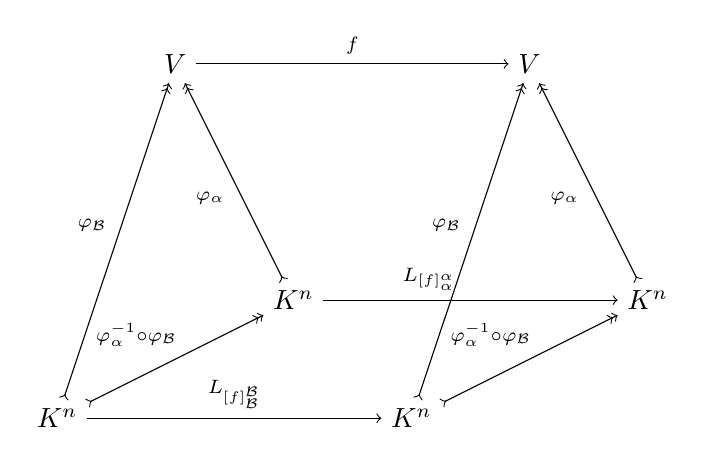
\begin{tikzpicture}[auto] 

    \node (a) at (0, 0) {$K^n $};
    \node (b) at (4.5, 0) {$K^n $};
    \node (c) at (3, 1.5) {$K^n $};
    \node (d) at (7.5, 1.5) {$K^n $};
    \node (e) at (1.5, 4.5) {$V$};
    \node (f) at (6, 4.5) {$V$};
    
    \draw [->] (a) to node {$\scriptstyle L_{\left[ f\right] _{\mathcal B}^{\mathcal B} } $} (b);
    \draw [->] (c) to node[xshift=-15pt, yshift=0pt] {$\scriptstyle L_{\left[ f\right] _{\alpha }^{\alpha } } $} (d);
    \draw [->] (e) to node {$\scriptstyle f$} (f);
    \draw [>->>] (a) to node {$\scriptstyle \varphi_{\mathcal B} $} (e);
    \draw [>->>] (b) to node {$\scriptstyle \varphi_{\mathcal B} $} (f);
    \draw [>->>] (c) to node {$\scriptstyle \varphi_{\alpha } $} (e);
    \draw [>->>] (d) to node {$\scriptstyle \varphi_{\alpha } $} (f);
    \draw [>->>] (a) to node[xshift=4pt, yshift=1pt] {$\scriptstyle \varphi_{\alpha }^{-1} \circ \varphi_{\mathcal B} $} (c);
    \draw [>->>] (b) to node[xshift=4pt, yshift=1pt] {$\scriptstyle \varphi_{\alpha }^{-1} \circ \varphi_{\mathcal B} $} (d);
    
  \end{tikzpicture} 
\end{center}
その写像$\varphi_{\alpha}^{- 1} \circ \varphi_{\mathcal{B}}$も線形同型写像であり、これに対応する行列を$P$とおくと、その行列$P$は正則行列であり次式のようになる。
\begin{center}
  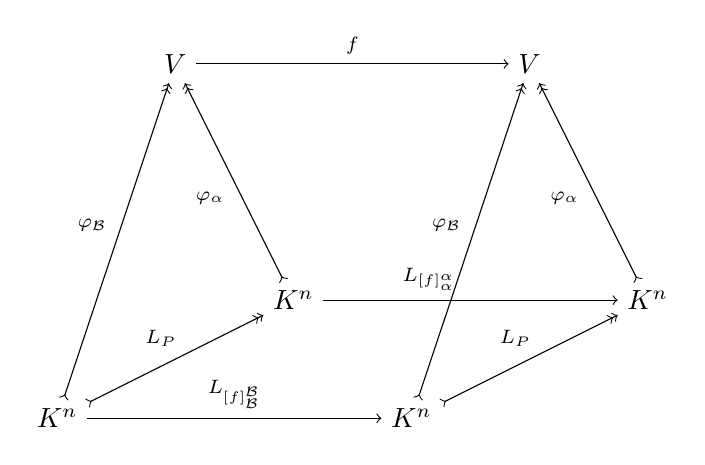
\begin{tikzpicture}[auto] 

    \node (a) at (0, 0) {$K^n $};
    \node (b) at (4.5, 0) {$K^n $};
    \node (c) at (3, 1.5) {$K^n $};
    \node (d) at (7.5, 1.5) {$K^n $};
    \node (e) at (1.5, 4.5) {$V$};
    \node (f) at (6, 4.5) {$V$};
    
    \draw [->] (a) to node {$\scriptstyle L_{\left[ f\right] _{\mathcal B}^{\mathcal B} } $} (b);
    \draw [->] (c) to node[xshift=-15pt, yshift=0pt] {$\scriptstyle L_{\left[ f\right] _{\alpha }^{\alpha } } $} (d);
    \draw [->] (e) to node {$\scriptstyle f$} (f);
    \draw [>->>] (a) to node {$\scriptstyle \varphi_{\mathcal B} $} (e);
    \draw [>->>] (b) to node {$\scriptstyle \varphi_{\mathcal B} $} (f);
    \draw [>->>] (c) to node {$\scriptstyle \varphi_{\alpha } $} (e);
    \draw [>->>] (d) to node {$\scriptstyle \varphi_{\alpha } $} (f);
    \draw [>->>] (a) to node[xshift=4pt, yshift=1pt] {$\scriptstyle L_P $} (c);
    \draw [>->>] (b) to node[xshift=4pt, yshift=1pt] {$\scriptstyle L_P $} (d);
    
  \end{tikzpicture} 
\end{center}
これにより、次のようになる。
\begin{align*}
L_{[ f]_{\mathcal{B}}^{\mathcal{B}}} = L_{P}^{- 1} \circ L_{[ f]_{\alpha}^{\alpha}} \circ L_{P} = L_{P^{- 1}[ f]_{\alpha}^{\alpha}P}
\end{align*}
よって、その基底$\alpha$に関するその線形写像$f$の表現行列$[ f]_{\alpha}^{\alpha}$を用いた行列$P^{- 1}[ f]_{\alpha}^{\alpha}P$も対角行列となる。\par
逆に、任意のそのvector空間$V$の基底$\alpha$に対し、$\exists P \in {\mathrm{GL} }_{n}(K)$に対し、その基底$\alpha$に関するその線形写像$f$の表現行列$[ f]_{\alpha}^{\alpha}$を用いた行列$P^{- 1}[ f]_{\alpha}^{\alpha}P$も対角行列となるとき、次式のようになる。
\begin{center}
  \begin{tikzpicture}[auto] 

    \node (a) at (0, 0) {$K^n $};
    \node (b) at (4.5, 0) {$K^n $};
    \node (c) at (3, 1.5) {$K^n $};
    \node (d) at (7.5, 1.5) {$K^n $};
    \node (e) at (1.5, 4.5) {$V$};
    \node (f) at (6, 4.5) {$V$};
    
    \draw [->] (a) to node {$\scriptstyle L_{P^{-1} \left[ f\right] _{\alpha }^{\alpha } P} $} (b);
    \draw [->] (c) to node[xshift=-15pt, yshift=0pt] {$\scriptstyle L_{\left[ f\right] _{\alpha }^{\alpha } } $} (d);
    \draw [->] (e) to node {$\scriptstyle f$} (f);
    \draw [>->>] (c) to node {$\scriptstyle \varphi_{\alpha } $} (e);
    \draw [>->>] (d) to node {$\scriptstyle \varphi_{\alpha } $} (f);
    \draw [>->>] (a) to node[xshift=4pt, yshift=1pt] {$\scriptstyle L_P $} (c);
    \draw [>->>] (b) to node[xshift=4pt, yshift=1pt] {$\scriptstyle L_P $} (d);
    
  \end{tikzpicture} 
\end{center}
ここで、合成写像$\varphi_{\alpha} \circ L_{P}:K^{n} \rightarrow V$を$\varphi_{\mathcal{B}}$とおくと、定理\ref{2.1.5.1}より次式のようになり、
\begin{center}
  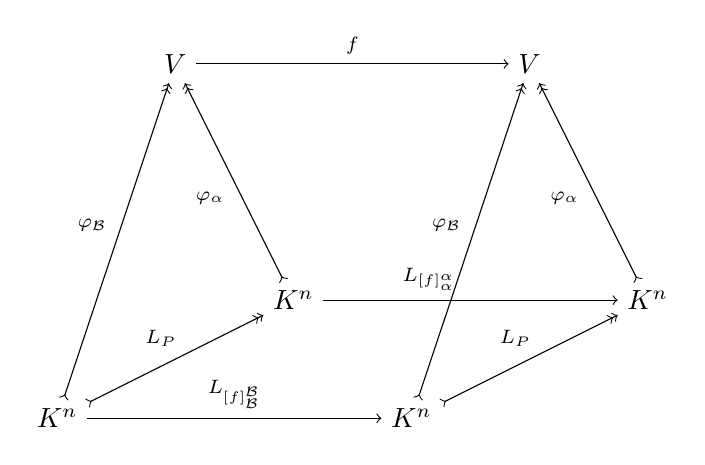
\begin{tikzpicture}[auto] 

    \node (a) at (0, 0) {$K^n $};
    \node (b) at (4.5, 0) {$K^n $};
    \node (c) at (3, 1.5) {$K^n $};
    \node (d) at (7.5, 1.5) {$K^n $};
    \node (e) at (1.5, 4.5) {$V$};
    \node (f) at (6, 4.5) {$V$};
    
    \draw [->] (a) to node {$\scriptstyle L_{\left[ f\right] _{\mathcal B}^{\mathcal B} } $} (b);
    \draw [->] (c) to node[xshift=-15pt, yshift=0pt] {$\scriptstyle L_{\left[ f\right] _{\alpha }^{\alpha } } $} (d);
    \draw [->] (e) to node {$\scriptstyle f$} (f);
    \draw [>->>] (a) to node {$\scriptstyle \varphi_{\mathcal B} $} (e);
    \draw [>->>] (b) to node {$\scriptstyle \varphi_{\mathcal B} $} (f);
    \draw [>->>] (c) to node {$\scriptstyle \varphi_{\alpha } $} (e);
    \draw [>->>] (d) to node {$\scriptstyle \varphi_{\alpha } $} (f);
    \draw [>->>] (a) to node[xshift=4pt, yshift=1pt] {$\scriptstyle L_P $} (c);
    \draw [>->>] (b) to node[xshift=4pt, yshift=1pt] {$\scriptstyle L_P $} (d);
    
  \end{tikzpicture} 
\end{center}
よって、そのvector空間$V$の線形写像$f:V \rightarrow V$のある基底$\mathcal{B}$が存在してこれに関するその線形写像$f$の表現行列$[ f]_{\mathcal{B}}^{\mathcal{B}}$が対角行列となるので、その線形写像$f$は対角化可能である。
\end{proof}
\begin{thm}\label{2.2.2.12}
体$K$上の$n$次元vector空間$V$の線形写像$f:V \rightarrow V$がその基底$\mathcal{B}$で対角化可能であるならそのときに限り、$\forall i \in \varLambda_{n}$に対し、その基底$\mathcal{B}$をなすvector$\mathbf{v}_{i}$がいずれもその線形写像$f$の固有値$\lambda_{i}$に対する固有vectorsである。このとき、その基底$\mathcal{B}$に関するその線形写像$f$の表現行列$[ f]_{\mathcal{B}}^{\mathcal{B}}$が次式のように与えられる。
\begin{align*}
[ f]_{\mathcal{B}}^{\mathcal{B}} = \begin{pmatrix}
\lambda_{1} & \  & \  & O \\
\  & \lambda_{2} & \  & \  \\
\  & \  & \ddots & \  \\
O & \  & \  & \lambda_{n} \\
\end{pmatrix}
\end{align*}
\end{thm}
\begin{proof}
体$K$上の$n$次元vector空間$V$の線形写像$f:V \rightarrow V$がその基底$\mathcal{B}$で対角化可能であるなら、その線形写像$f$のその基底$\mathcal{B}$に関する表現行列$[ f]_{\mathcal{B}}^{\mathcal{B}}$が対角行列であり、次式のようにおき
\begin{align*}
[ f]_{\mathcal{B}}^{\mathcal{B}} = \begin{pmatrix}
\lambda_{1} & \  & \  & O \\
\  & \lambda_{2} & \  & \  \\
\  & \  & \ddots & \  \\
O & \  & \  & \lambda_{n} \\
\end{pmatrix}
\end{align*}
$\mathcal{B} =\left\langle \mathbf{v}_{i} \right\rangle_{i \in \varLambda_{n}}$とおくと、定理\ref{2.1.5.1}よりその基底$\mathcal{B}$に関する基底変換における線形同型写像$\varphi_{\mathcal{B}}:K^{n} \rightarrow V$は線形同型写像であり次式が成り立つので、
\begin{center}
  \begin{tikzpicture}[auto]

    \node (a) at (0, 0) {$K^n $};
    \node (b) at (3, 0) {$K^n $};
    \node (c) at (0, 3) {$V$};
    \node (d) at (3, 3) {$V$};
    
    \draw [->] (a) to node {$\scriptstyle L_{\left[ f\right]_{\mathcal B}^{\mathcal B}} $} (b);
    \draw [->] (c) to node {$\scriptstyle f$} (d);
    \draw [>->>] (a) to node {$\scriptstyle \varphi_{\mathcal B} $} (c);
    \draw [>->>] (b) to node {$\scriptstyle \varphi_{\mathcal B} $} (d);
    
  \end{tikzpicture} 
\end{center}
$\forall i \in \varLambda_{n}$に対し、vector空間$K^{n}$の正規直交基底を$\left\langle \mathbf{e}_{i} \right\rangle_{i \in \varLambda_{n}}$とおくと、次のようになる。
\begin{align*}
f\left( \mathbf{v}_{i} \right) &= \varphi_{\mathcal{B}} \circ L_{[ f]_{\mathcal{B}}^{\mathcal{B}}} \circ \varphi_{\mathcal{B}}^{- 1}\left( \mathbf{v}_{i} \right)\\
&= \varphi_{\mathcal{B}}\left( L_{[ f]_{\mathcal{B}}^{\mathcal{B}}}\left( \varphi_{\mathcal{B}}^{- 1}\left( \mathbf{v}_{i} \right) \right) \right)\\
&= \varphi_{\mathcal{B}}\left( L_{[ f]_{\mathcal{B}}^{\mathcal{B}}}\left( \mathbf{e}_{i} \right) \right)\\
&= \varphi_{\mathcal{B}}\left( [ f]_{\mathcal{B}}^{\mathcal{B}}\mathbf{e}_{i} \right)\\
&= \varphi_{\mathcal{B}}\left( \begin{pmatrix}
\lambda_{1} & \  & \  & \  & \  & O \\
\  & \lambda_{2} & \  & \  & \  & \  \\
\  & \  & \ddots & \  & \  & \  \\
\  & \  & \  & \lambda_{i} & \  & \  \\
\  & \  & \  & \  & \ddots & \  \\
O & \  & \  & \  & \  & \lambda_{n} \\
\end{pmatrix}\begin{pmatrix}
0 \\
0 \\
 \vdots \\
1 \\
 \vdots \\
0 \\
\end{pmatrix} \right)\\
&= \varphi_{\mathcal{B}}\begin{pmatrix}
0 \\
0 \\
 \vdots \\
\lambda_{i} \\
 \vdots \\
0 \\
\end{pmatrix}\\
&= \varphi_{\mathcal{B}}\left( \lambda_{i}\mathbf{e}_{i} \right)\\
&= \lambda_{i}\varphi_{\mathcal{B}}\left( \mathbf{e}_{i} \right) = \lambda_{i}\mathbf{v}_{i}
\end{align*}
よって、その基底$\mathcal{B}$をなすvectorsがいずれもその線形写像$f$の固有vectorsである。\par
逆に、$\forall i \in \varLambda_{n}$に対し、その基底$\mathcal{B}$をなすvector$\mathbf{v}_{i}$がいずれもその線形写像$f$の固有値$\lambda_{i}$に対する固有vectorsであるなら、$f\left( \mathbf{v}_{i} \right) = \lambda_{i}\mathbf{v}_{i}$が成り立つことになる。ここで、定理\ref{2.1.5.1}よりその基底$\mathcal{B}$に関する基底変換における線形同型写像$\varphi_{\mathcal{B}}:K^{n} \rightarrow V$について、次式が成り立つので、
\begin{center}
  \begin{tikzpicture}[auto]

    \node (a) at (0, 0) {$K^n $};
    \node (b) at (3, 0) {$K^n $};
    \node (c) at (0, 3) {$V$};
    \node (d) at (3, 3) {$V$};
    
    \draw [->] (a) to node {$\scriptstyle L_{\left[ f\right]_{\mathcal B}^{\mathcal B}} $} (b);
    \draw [->] (c) to node {$\scriptstyle f$} (d);
    \draw [>->>] (a) to node {$\scriptstyle \varphi_{\mathcal B} $} (c);
    \draw [>->>] (b) to node {$\scriptstyle \varphi_{\mathcal B} $} (d);
    
  \end{tikzpicture} 
\end{center}
$\forall\sum_{i \in \varLambda_{n}} {a_{i}\mathbf{e}_{i}} \in K^{n}$に対し、次のようになる。
\begin{align*}
L_{[ f]_{\mathcal{B}}^{\mathcal{B}}}\left( \sum_{i \in \varLambda_{n}} {a_{i}\mathbf{e}_{i}} \right) &= \sum_{i \in \varLambda_{n}} {a_{i}f\left( \mathbf{e}_{i} \right)}\\
&= \sum_{i \in \varLambda_{n}} {a_{i}\varphi_{\mathcal{B}}^{- 1} \circ f \circ \varphi_{\mathcal{B}}\left( \mathbf{e}_{i} \right)}\\
&= \sum_{i \in \varLambda_{n}} {a_{i}\varphi_{\mathcal{B}}^{- 1}\left( f\left( \varphi_{\mathcal{B}}\left( \mathbf{e}_{i} \right) \right) \right)}\\
&= \sum_{i \in \varLambda_{n}} {a_{i}\varphi_{\mathcal{B}}^{- 1}\left( f\left( \mathbf{v}_{i} \right) \right)}\\
&= \sum_{i \in \varLambda_{n}} {a_{i}\varphi_{\mathcal{B}}^{- 1}\left( \lambda_{i}\mathbf{v}_{i} \right)}\\
&= \sum_{i \in \varLambda_{n}} {a_{i}\lambda_{i}\mathbf{e}_{i}}\\
&= \sum_{i \in \varLambda_{n}} \begin{pmatrix}
0 \\
0 \\
 \vdots \\
a_{i}\lambda_{i} \\
 \vdots \\
0 \\
\end{pmatrix}\\
&= \begin{pmatrix}
\lambda_{1}\mathbf{e}_{1} & \lambda_{2}\mathbf{e}_{2} & \cdots & \lambda_{n}\mathbf{e}_{n} \\
\end{pmatrix}\begin{pmatrix}
a_{1} \\
a_{2} \\
 \vdots \\
a_{n} \\
\end{pmatrix}\\
&= \begin{pmatrix}
\lambda_{1} & \  & \  & O \\
\  & \lambda_{2} & \  & \  \\
\  & \  & \ddots & \  \\
O & \  & \  & \lambda_{n} \\
\end{pmatrix}\begin{pmatrix}
a_{1} \\
a_{2} \\
 \vdots \\
a_{n} \\
\end{pmatrix}
\end{align*}
よって、その基底$\mathcal{B}$に関するその線形写像$f$の表現行列$[ f]_{\mathcal{B}}^{\mathcal{B}}$が次式のように対角行列となるので、
\begin{align*}
[ f]_{\mathcal{B}}^{\mathcal{B}} = \begin{pmatrix}
\lambda_{1} & \  & \  & O \\
\  & \lambda_{2} & \  & \  \\
\  & \  & \ddots & \  \\
O & \  & \  & \lambda_{n} \\
\end{pmatrix}
\end{align*}
その線形写像$f$はその基底$\mathcal{B}$で対角化可能である。
\end{proof}
\begin{thm}\label{2.2.2.13}
体$K$上の有限次元なvector空間$V$の線形写像$f:V \rightarrow V$の添数集合$\varLambda_{n}$によって添数づけられた互いに異なる固有値たちからなる族$\left\{ \lambda_{i} \right\}_{i \in \varLambda_{n}}$が与えられたとき、$\forall i \in \varLambda_{n}$に対し、その固有値$\lambda_{i}$に対する固有vectorのうち1つを$\mathbf{v}_{i}$とおくと、その族$\left\{ \mathbf{v}_i \right\}_{i \in \varLambda_{n} }$は線形独立である。
\end{thm}
\begin{proof}
体$K$上の有限次元なvector空間$V$の線形写像$f:V \rightarrow V$の添数集合$\varLambda_{n}$によって添数づけられた互いに異なる固有値たちからなる族$\left\{ \lambda_{i} \right\}_{i \in \varLambda_{n}}$が与えられたとき、$\forall i \in \varLambda_{n}$に対し、その固有値$\lambda_{i}$に対する固有vectorのうち1つを$\mathbf{v}_{i}$とおくと、$n = 1$のときは明らかにであるから、$n = k$のとき、その族$\left\{ \mathbf{v}_i \right\}_{i \in \varLambda_{k}}$は線形独立であると仮定しよう。$n = k + 1$のとき、$i \in \varLambda_{k + 1}$なる体$K$の元々$c_{i}$を用いて次式が成り立つとすれば、
\begin{align*}
\sum_{i \in \varLambda_{k + 1}} {c_{i}\mathbf{v}_{i}} = \mathbf{0}
\end{align*}
次のようになる。
\begin{align*}
\sum_{i \in \varLambda_{k + 1}} {c_{i}\mathbf{v}_{i}} = \mathbf{0} &\Leftrightarrow \sum_{i \in \varLambda_{k + 1}} {c_{i}\mathbf{v}_{i}} = \mathbf{0} \land f\left( \sum_{i \in \varLambda_{k + 1}} {c_{i}\mathbf{v}_{i}} \right) = f\left( \mathbf{0} \right)\\
&\Leftrightarrow \sum_{i \in \varLambda_{k + 1}} {c_{i}\mathbf{v}_{i}} = \mathbf{0} \land \sum_{i \in \varLambda_{k + 1}} {c_{i}f\left( \mathbf{v}_{i} \right)} = \mathbf{0}\\
&\Leftrightarrow \sum_{i \in \varLambda_{k + 1}} {c_{i}\lambda_{k + 1}\mathbf{v}_{i}} = \mathbf{0} \land \sum_{i \in \varLambda_{k + 1}} {c_{i}\lambda_{i}\left( \mathbf{v}_{i} \right)} = \mathbf{0}\\
&\Leftrightarrow \sum_{i \in \varLambda_{k}} {c_{i}\lambda_{k + 1}\mathbf{v}_{i}} + c_{k + 1}\lambda_{k + 1}\mathbf{v}_{k + 1} = \mathbf{0} \land \sum_{i \in \varLambda_{k}} {c_{i}\lambda_{i}\left( \mathbf{v}_{i} \right)} + c_{k + 1}\lambda_{k + 1}\mathbf{v}_{k + 1} = \mathbf{0}\\
&\Rightarrow \left( \sum_{i \in \varLambda_{k}} {c_{i}\lambda_{k + 1}\mathbf{v}_{i}} + c_{k + 1}\lambda_{k + 1}\mathbf{v}_{k + 1} \right) - \left( \sum_{i \in \varLambda_{k}} {c_{i}\lambda_{i}\left( \mathbf{v}_{i} \right)} + c_{k + 1}\lambda_{k + 1}\mathbf{v}_{k + 1} \right) = \mathbf{0}\\
&\Leftrightarrow \sum_{i \in \varLambda_{k}} {c_{i}\lambda_{k + 1}\mathbf{v}_{i}} + c_{k + 1}\lambda_{k + 1}\mathbf{v}_{k + 1} - \sum_{i \in \varLambda_{k}} {c_{i}\lambda_{i}\left( \mathbf{v}_{i} \right)} - c_{k + 1}\lambda_{k + 1}\mathbf{v}_{k + 1} = \mathbf{0}\\
&\Leftrightarrow \sum_{i \in \varLambda_{k}} {c_{i}\left( \lambda_{k + 1} - \lambda_{i} \right)\mathbf{v}_{i}} = \mathbf{0}
\end{align*}
ここで、仮定より$\forall i \in \varLambda_{k}$に対し、$c_{i}\left( \lambda_{k + 1} - \lambda_{i} \right) = 0$が成り立つので、$c_{i} = 0$または$\lambda_{i} = \lambda_{k + 1}$が成り立ち、仮定より$c_{i} = 0$が成り立つ。これにより、次のようになる。
\begin{align*}
\sum_{i \in \varLambda_{k + 1}} {c_{i}\mathbf{v}_{i}} &= \sum_{i \in \varLambda_{k}} {c_{i}\mathbf{v}_{i}} + c_{k + 1}\mathbf{v}_{k + 1}\\
&= \sum_{i \in \varLambda_{k}} \mathbf{0} + c_{k + 1}\mathbf{v}_{k + 1}\\
&= c_{k + 1}\mathbf{v}_{k + 1} = \mathbf{0}
\end{align*}
ここで、そのvector$\mathbf{v}_{k + 1}$は固有vectorの定義より零vectorでないので、$c_{k + 1} = 0$が成り立つ。\par
以上より、数学的帰納法によって$\forall i \in \varLambda_{n}$に対し、$c_{i} = 0$が成り立ち、その族$\left\{ \mathbf{v}_i \right\}_{i \in \varLambda_{n} } $に対するvectors$\mathbf{v}_{i}$は線形独立である。
\end{proof}
%\hypertarget{ux56faux6709ux7a7aux9593}{%
\subsubsection{固有空間}%\label{ux56faux6709ux7a7aux9593}}
\begin{dfn} 定理\ref{2.2.2.2}より体$K$上のvector空間$V$の元$\mathbf{v}$が線形写像$f:V \rightarrow V$の固有値$\lambda$に対する固有vectorであるならそのときに限り、そのvector$\mathbf{v}$はその集合$\ker\left( \lambda I_{V} - f \right) \setminus \left\{ \mathbf{0} \right\}$の元であるのであった。ここで、次式のように集合$W_{f}(\lambda)$が定義され、その集合$W_{f}(\lambda)$をその固有値$\lambda$に対する固有空間という。
\begin{align*}
W_{f}(\lambda) = \ker\left( \lambda I_{V} - f \right)
\end{align*}
\end{dfn}
\begin{thm}\label{2.2.2.14}
体$K$上のvector空間$V$の線形写像$f:V \rightarrow V$の固有値$\lambda$に対する固有空間$W_{f}(\lambda)$はそのvector空間$V$の部分空間である。
\end{thm}
\begin{proof} 固有空間の定義と定理\ref{2.1.2.11}より直ちに示される。
\end{proof}
\begin{thm}\label{2.2.2.15}
体$K$上の有限次元なvector空間$V$の線形写像$f:V \rightarrow V$の添数集合$\varLambda_{n}$によって添数づけられた互いに異なる固有値たちからなる族$\left\{ \lambda_{i} \right\}_{i \in \varLambda_{n}}$が与えられたとき、添数集合$\varLambda_{n}$によって添数づけられたそれらの固有値たち$\lambda_{i}$に対する固有空間$W_{f}\left( \lambda_{i} \right)$の族$\left\{ W_{f}\left( \lambda_{i} \right) \right\}_{i \in \varLambda_{n}}$の和空間$\sum_{i \in \varLambda_{n}} {W_{f}\left( \lambda_{i} \right)}$は直和空間$\bigoplus_{i \in \varLambda_{n}} {W_{f}\left( \lambda_{i} \right)}$でもある。
\end{thm}
\begin{proof}
体$K$上の有限次元なvector空間$V$の線形写像$f:V \rightarrow V$の添数集合$\varLambda_{n}$によって添数づけられた互いに異なる固有値たちからなる族$\left\{ \lambda_{i} \right\}_{i \in \varLambda_{n}}$が与えられたとき、添数集合$\varLambda_{n}$によって添数づけられたそれらの固有値たち$\lambda_{i}$に対する固有空間$W_{f}\left( \lambda_{i} \right)$の族$\left\{ W_{f}\left( \lambda_{i} \right) \right\}_{i \in \varLambda_{n}}$の和空間$\sum_{i \in \varLambda_{n}} {W_{f}\left( \lambda_{i} \right)}$について、$\forall\mathbf{z} \in \sum_{i \in \varLambda_{n}} {W_{f}\left( \lambda_{i} \right)}$に対し、$\mathbf{z} = \sum_{i \in \varLambda_{n}} \mathbf{v}_{i} = \sum_{i \in \varLambda_{n}} \mathbf{v}_{i}'$なるその集合$\prod_{i \in \varLambda_{n}} {W_{f}\left( \lambda_{i} \right)}$の互いに異なる元々$\left( \mathbf{v}_{i} \right)_{i \in \varLambda_{n}}$、$\left( \mathbf{v}_{i}' \right)_{i \in \varLambda_{n}}$が存在すると仮定すると、次のようになる。
\begin{align*}
\sum_{i \in \varLambda_{n}} \left( \mathbf{v}_{i} - \mathbf{v}_{i}' \right) &= \sum_{i \in \varLambda_{n}} \mathbf{v}_{i} - \sum_{i \in \varLambda_{n}} \mathbf{v}_{i}'\\
&= \mathbf{z} - \mathbf{z} = \mathbf{0}
\end{align*}
ここで、$\mathbf{v}_{i} - \mathbf{v}_{i}' \in W_{f}\left( \lambda_{i} \right)$が成り立ち、定理\ref{2.2.2.13}より$\forall i \in \varLambda_{n}$に対し、その固有値$\lambda_{i}$に対する固有vectors$\mathbf{v}_{i}$は線形独立であるので、$\forall i \in \varLambda_{n}$に対し、それらのvectors$\mathbf{v}_{i} - \mathbf{v}_{i}'$は固有vectorでないことになる。したがって、それらのvectors$\mathbf{v}_{i} - \mathbf{v}_{i}'$は零vectorsであり、$\forall i \in \varLambda_{n}$に対し、$\mathbf{v}_{i} = \mathbf{v}_{i}'$が成り立つ。しかしながら、これは仮定に矛盾する。したがって、$\forall\mathbf{z} \in \sum_{i \in \varLambda_{n}} {W_{f}\left( \lambda_{i} \right)}$に対し、$\mathbf{z} = \sum_{i \in \varLambda_{n}} \mathbf{v}_{i}$なるその集合$\prod_{i \in \varLambda_{n}} {W_{f}\left( \lambda_{i} \right)}$の元$\left( \mathbf{v}_{i} \right)_{i \in \varLambda_{n}}$が一意的に存在することになり、直和空間の定義よりその和空間$\sum_{i \in \varLambda_{n}} {W_{f}\left( \lambda_{i} \right)}$は直和空間$\bigoplus_{i \in \varLambda_{n}} {W_{f}\left( \lambda_{i} \right)}$でもある。
\end{proof}
\begin{thebibliography}{50}
  \bibitem{1}
    松坂和夫, 線型代数入門, 岩波書店, 1980. 新装版第2刷 p226-246 ISBN978-4-00-029872-8
  \bibitem{2}
    対馬龍司, 線形代数学講義, 共立出版, 2007. 改訂版8刷 p155-164 ISBN978-4-320-11097-7
\end{thebibliography}
\end{document}
